\documentclass[a4j,11pt,report]{jsbook}
\usepackage[dvipdfmx]{graphicx}
\usepackage{tabularx}
\usepackage{fancybox}
\usepackage{ascmac}
\usepackage{amsmath,amssymb,amsthm}
\usepackage[dviout]{graphicx}
\usepackage{subcaption}
\setlength{\topmargin}{-1in}
\addtolength{\topmargin}{5mm}
\setlength{\headheight}{5mm}
\setlength{\headsep}{0mm}
\setlength{\textheight}{\paperheight}
\addtolength{\textheight}{-25mm}
\setlength{\footskip}{5mm}

\newcommand{\frontpage}[3]{%
\title{卒業論文\\ \vspace{3em}\\{\huge #1}\\ \\#2\vspace{15em}}%
\author{{\huge 成蹊大学理工学部情報科学科}\\ \\{\huge #3}}%
\date{}
\maketitle
\clearpage
\thispagestyle{empty}

\clearpage
}



\newcommand{\point}[1]{
\begin{itembox}[l]{ポイント}
  #1
\end{itembox}
}

\begin{document}

\frontpage  % 以下の各項目を自分のテーマにあわせて修正する.
{計算問題の特徴分布に基づく類題選出による自己学習支援}
{Self Learning Support by Automatic Selection of Calculation Exercises based on Feature Distribution of Exercises}
{S152114 宮地 雄也}

\chapter*{要旨}
\thispagestyle{empty}
\point{
序論と結論の内容をもとに研究の内容をまとめる.
\begin{itemize}
  \item 問いは何か??
  \item 主張は何か??
  \item 結果はどうだったのか?
  \item 得られた成果の意義は?
\end{itemize}
}

\tableofcontents
\thispagestyle{empty}
\clearpage
\thispagestyle{plain}
\setcounter{page}{1}

\chapter{序論 \label{ch:introduction}}

\point{
問題提起を行う.
解く価値があり,簡単には解けず,誰も解いていない問題を扱っていることがわかるようにする.
\begin{itemize}
  \item どういう問題に取り組んだのか?
  \item その問題を解くことがなぜ重要なのか? 社会的意義(有用性)・学術的意義(問題の面白さ)
  \item その問題はどこが難しいのか? なぜこれまで解かれていなかったのか? これまではどうしていたのか?
  \item その問題をどのようなアプローチで解こうとしたのか? なぜそうしたのか?
\end{itemize}
}

\section{memo}
近年,子供達一人一人に目を向けたアダプティブラーニングが注目を集めていますが,現在の日本の教育現場では集合教育が基本であり
一人一人に対応するのは難しい.また教員の働き方にも是正が求められていて,仮に個々に対応しようとすると労働時間外になってしまう.
そこで個人最適化した学習を情報技術で叶えようとする動きが活発である.
そこで私は間違えた問いに対して復習問題を出す際,その数式の特徴を捉えて類題が作れないかと考えた.
今までは問題をといた子供達の集合に目を向けられていたが,本論文では数式自体に目を向け類似する問題を作り出そうとした.
本論文では数式の特徴を掴むために自然言語処理の分野で使用される分散表現を適用し,さらに再起ニューラルネットワークを用いて数式ベクトルを作り出すことを目標とし,そのベクトルを用いて実際に復習問題生成を行った.




\chapter{背景知識\label{ch:background}}

\point{
以降の内容を理解するための準備を行う.
\begin{itemize}
  \item 章題は適切なものに変えること.章をわけてもよい.
  \item 以降の説明で用いる専門用語・表記法を説明する.
  \item 以降の内容を理解するのに必要となる,技術や理論を説明する.
\end{itemize}
}
\section{現在の小中教育業界の現状}
忙しいことをとにかく集める.なんなら塾の観点でも.
子供の減少にも

\section{アダプティブラーニング}

*******************************************

今世の中でどのようなことが行われているかを収集.
その手法を2,3事例あげて説明

*******************************************

アダプティブラーニングとは、学習者一人ひとりの学習進捗度(学習進度)に最適化された学習方法と学習教材を選択し、
提供する仕組みを持つ学習エンジンやシステム、ソフトウェア、サービスなどを統括的に指す言葉です。

アダプティブラーニングは、IT技術を教育分野に活用するEdTech(Education Technology)の1つとして世界中から多くの注目を集めています。
アダプティブラーニングの先駆企業であり世界中でシェアを獲得している米Knewton社CEOのライアン・プリチャード氏は、日本法人であるニュートンジャパン株式会社主催のアダプティブラーニングをテーマにしたイベント『Knewton Day Tokyo 2017- Adaptive Learning Summit -』のQ&Aセッション内で、アダプティブラーニングの定義について上記のように回答しました。
よって本論文中でも以下のように定義する.
\begin{quote}
  データをもとにパーソナライズされた経験を継続的に提供するもので、
  生徒がシステムを使うたびにコンテンツやモデルをアップデートし、最適な道筋をアップデートするもの
\end{quote}

日本国内では

\section{ニューラルネットワーク}

*******************

きほんから!シナプスの話から流れを剃って数式,図つきで!

*******************

ニューラルネットワークのニューラルとは,生物のニューロン(神経細胞)に由来する.
ニューロンは、細胞核のある「細胞体」,他の細胞からの入力を受ける「樹状突起」,他の細胞に出力する「軸索」に分けられ,
ニューロンに入力刺激が入ってきた際に,ある一定以上の電圧であれば次のニューロンに刺激を伝えるという仕組みになっている.
また各軸索の太さは一定ではなく,何度も神経間のやり取りがなされたものは太くなり,情報伝達の優先度が高くなる.
この脳の仕組みを参考に考えられた数理モデルがニューラルネットワークである.

ニューラルネットではユニット(unit)と呼ばれる素子からなり,一つのユニットに複数の実数値の入力$x$があり,各入力に対して結合強度の重みをかけて出力$z$を算出します.
この一つのユニットをパーセプトロンという.(図\ref{fig:parceptron_image}参照)
このパーセプトロンのユニットを複数個かつ数段にわたり層状につなぎ合わせたアーキテクチャを順伝播型ニューラルネットワーク(Feedforward neural netwark)(図\ref{fig:NeuralNet_image}参照)と言う.
一般にニューラルネットワークと呼ばれるのはこの順伝播型を指しており,本論文でも単にニューラルネットワークと言った場合はこれのことをさす.

\begin{figure}[ht]
  \centering
  \begin{subfigure}{0.4\columnwidth }
    \centering
    
\includegraphics[width=\columnwidth ]{image/NeuralNet_parceptron.png}
    \caption{パーセプトロン模式図}
    \label{fig:parceptron_image}
  \end{subfigure}

  \begin{subfigure}{0.4\columnwidth }
    \centering
    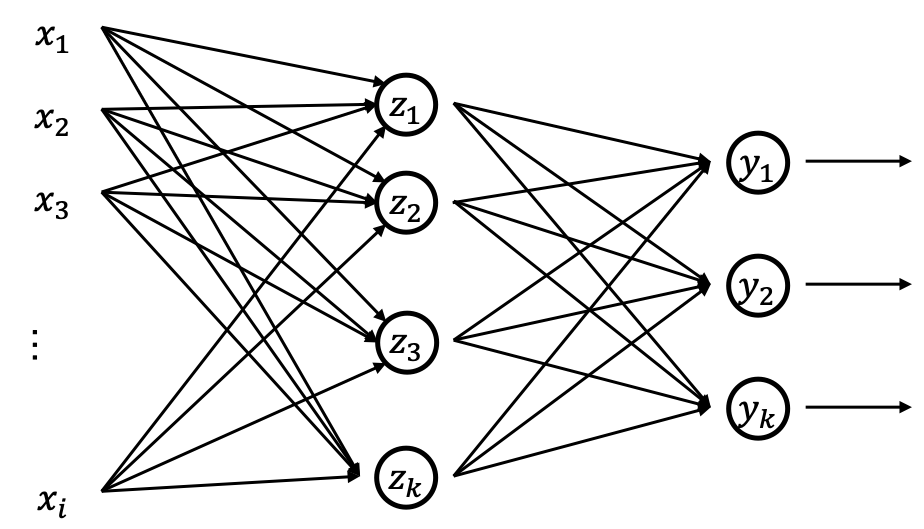
\includegraphics[width=\columnwidth]{image/forwardNeuralNetwork.png}
    \caption{ニューラルネットワーク模式図}
    \label{fig:NeuralNet_image}

  \end{subfigure}

\end{figure}


\section{分散表現}
様々な手法を紹介する
CBow,skipGram,GloVeなど
計算式を並べて最後にどこが長所で,どこが違うのかを表現
\section{畳み込みニューラルネットワーク}


\section{再起ニューラルネットワーク}

参照のニューラルネットがforwardNNなのに対しなぜ再起がいいのかを簡潔に
グラフを使いながら

\section{LSTM(Long short-term memory)}

再起を受けて通常のRNNでは叶わないところを明確に





\chapter{提案手法(章題は変える)\label{ch:method}}
\point{
自分の提案する解決方法を説明する.
\begin{itemize}
  \item 章題は適切なものに変えること.章をわけてもよい.
  \item 必ず具体例を用いること.
  \item 最初に問題を解く上で最も難しい点とそれを解決するアイデアを示す.
  \item 詳細については,全体の流れを示した後,各ステップについて説明する.
  \item 検討時に行った予備評価の結果があれば示す.
\end{itemize}
}

\section{流れ}
図をいれながら
\section{各システムの詳細}
\subsection{事前学習}

\subsubsection{丸ばつ判定の学習}
今回提案するシステムではといたプリントを読み込みその結果を判別して間違った計算問題を見つけ,その類題を選出する.

\begin{figure}[ht]
  \begin{center}
    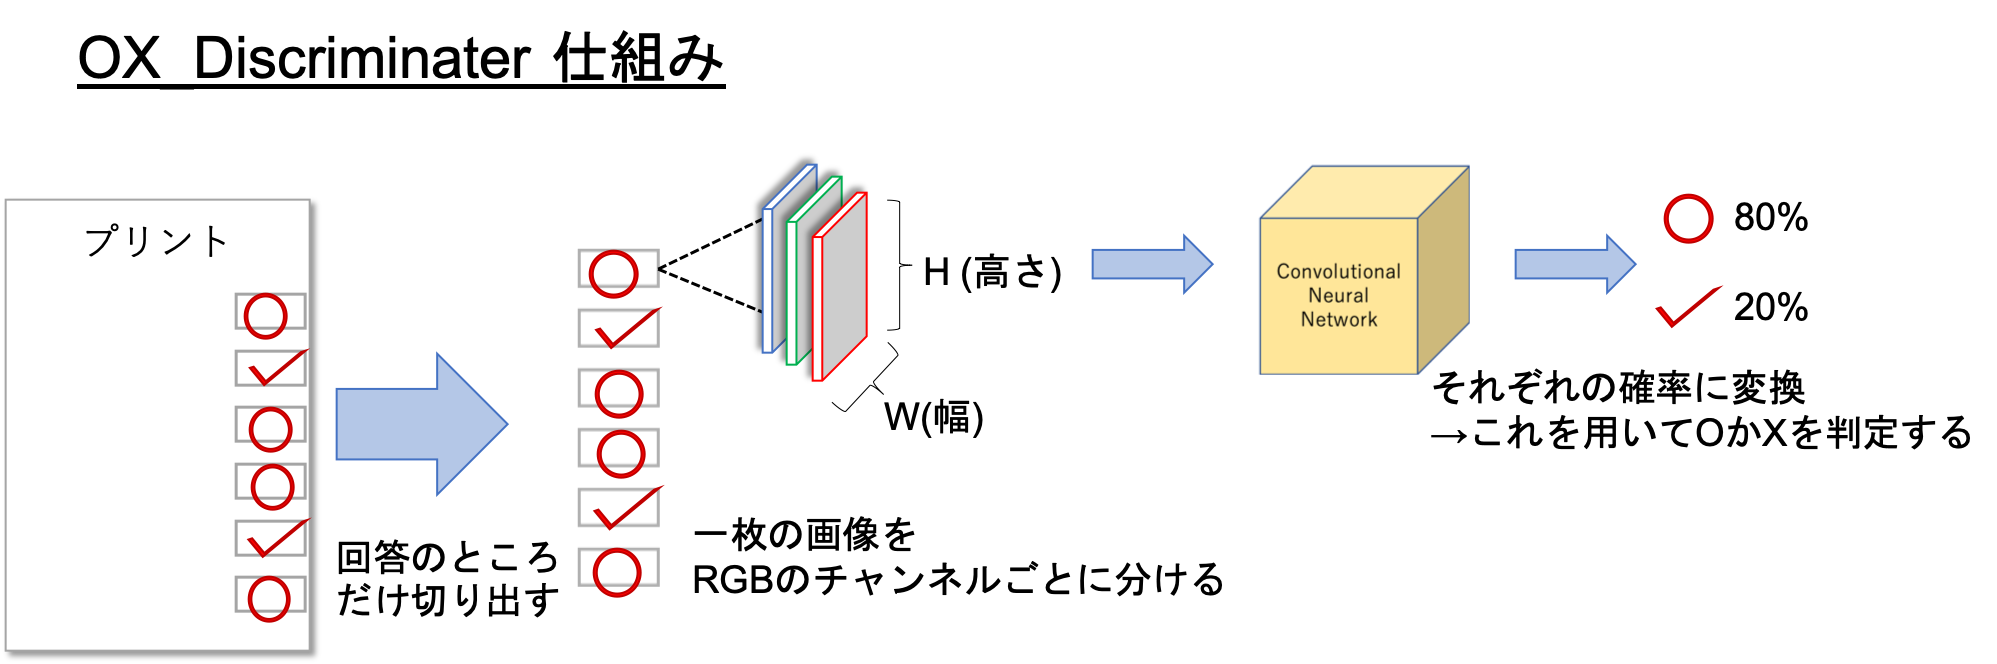
\includegraphics[width = 15cm]{image/OX_Discriminater.png}
    \caption{OX_Discriminaterイメージ図}
    \label{fig:OX_Discriminater_image}
  \end{center}
\end{figure}

\subsubsection{分散表現の事前学習}

\subsection{システム利用時の流れ}

\subsection{}
\subsection{}
\subsection{}
\subsection{}






\chapter{結果とその検討 \label{ch:result}}

\point{
自分の提案する方法が序論で提起した問題を解決できているかを評価・分析する.
\begin{itemize}
  \item 目的.何を確認するためのものか
  \item 方法.そのためにどういう実験を行ったか? 実験環境・用いたデータとその選定理由・手順を示し,評価の適切性を論証すること.
  \item 結果.その結果はどうだったか? 表やグラフを用いてまとめる.表はTeX,グラフはexcelでなくpythonを用いて作成すること.
  \item 分析.その結果から何が言えるか? 達成できた点・不足している点を理由と共に述べ,原因を考察する.
\end{itemize}
}

\chapter{関連研究\label{ch:relatedwork}}
\point{
この研究に関連する他の研究を紹介し,この研究との違いを明確にする.
\begin{itemize}
  \item 文献は「Mnihらは~という手法を提案している\cite{Mnih15}.」のように\texttt{cite}コマンドを用いて文献番号を示すこと.
  \item 2ページ以上書く.
\end{itemize}
}

\chapter{結論と今後の課題 \label{ch:conclusion}}

\point{
序論で提起した問いとそれに対する答えをまとめる.
\begin{itemize}
  \item 提案手法のアイデアおよび評価結果を振り返る.
  \item この研究で得られた知見をまとめる.
  \item 今後の課題について述べる.
\end{itemize}
}

\bibliographystyle{ipsjsort}
\bibliography{ref}

\appendix

\chapter{形式上の注意}

\begin{itemize}
  \item 文字コードはUTF-8に統一する.
  \item 論文ファイル名は\texttt{chishiro-thesis.tex},文献ファイル名は\texttt{chishiro.bib}のように名前\texttt{-thesis.tex}とする.
  \item 句読点は全角のカンマ,ピリオドを用いる.
  \item 英数字はすべて半角を用いる.ギリシャ文字は{\TeX}の定義を用いる.$\alpha, \beta, ...$
  \item カンマの前にはスペースを入れず,カンマの後はスペースをひとつ入れる.
  \item 数式は{\TeX}の数式機能を用いる.例: $x^2$,\[f(x) = x^2 + 2x + 1.\].
  \item プログラムテキストはタイプライターフォントを用いる(例: \texttt{hello}).
  \item 文章構成(章・節・小節・箇条書き)は{\TeX}の機能を用いて指定する.自分で見出しなどを作らない.
  \item 題目には研究目的・方法・対象を特徴づける情報を入れる.
  \item 図のタイトルは図の下,表のタイトルは表の上に書く.
  \item 図表番号の参照は\verb#\label#および\verb#\ref#を用いる.自分で図表番号を指定しない.
  \item 表は{\TeX},グラフはすべてpythonで作成する.
  \item 図表番号のない図は用いない.
  \item 参照の?は必ず取り除く.
  \item 段落は意味の区切りでわける.意図しない字下げが入った場合\verb#\noindent#を用いて修正する.
  \item 参考文献は10以上あげる.
\end{itemize}


\chapter*{謝辞 \label{ch:acknowledgement}}
\thispagestyle{empty}
\point{
本のあとがきに相当する部分.半ページ以上書く.
卒業研究に協力者してくれた方々へのお礼を忘れずに述べる.
}

卒業論文を書くにあたってたくさんの人に支えてもらった.
様々なアドバイスをしていただいた千代教授には心より,感謝を申し上げたい.
また共に四年間学んだ研究室メンバーにもたくさん支えられてこの論文書き上げることができた.
多くの学びとたくさんの思い出を共有できた研究室メンバーにも感謝したい.

また毎週,宿題と合わせて一次方程式のプリントを文句を言いながらもといてくれた栄光ゼミナール新船橋校の中学校1年の私のクラスの生徒がいなければ
この研究を行うこともできなかった.
彼らの勉強の足しになればと思い作り始めた追加プリントはたくさんの情報を教えてくれました.
一年間しか担当できませんでしたが,少しでも彼らの力になっていればなと思う.
この研究を糧に社会に出ても,たくさんの子供達が自ら学ぼうとする時,その障壁を共に歩み,打破するそんな気持ちの込もったコンテンツを作って行ければなと思い,末筆としたい.

\end{document}
